\protect\hyperlink{main-nav}{≡} \protect\hyperlink{close-nav}{×}

\hypertarget{section-4.3-optimization}{%
\section{Section 4.3: Optimization}\label{section-4.3-optimization}}

The partial derivatives tell us something about where a surface has
local maxima and minima. Remember that even in the one-variable cases,
there were critical points which were neither maxima nor minima -- this
is also true for functions of many variables. In fact, as you might
expect, the situation is even more complicated.

\hypertarget{second-derivatives}{%
\subsection{Second Derivatives}\label{second-derivatives}}

When you find a partial derivative of a function of two variables, you
get another function of two variables -- you can take its partial
derivatives, too. We've done this before, in the one-variable setting.
In the one-variable setting, the second derivative gave information
about how the graph was curved. In the two-variable setting, the second
partial derivatives give some information about how the surface is
curved, as you travel on cross-sections -- but that's not very complete
information about the entire surface.

Imagine that you have a surface that's ruffled around a point, like what
happens near a button on an overstuffed sofa, or a pinched piece of
fabric, or the wrinkly skin near your thumb when you make a fist. Right
at that point, every direction you move, something different will happen
-- it might increase, decrease, curve up, curve down\ldots{} A simple
phrase like ``concave up'' or ``concave down'' can't describe all the
things that can happen on a surface.

Surprisingly enough, though, there is still a second derivative test
that can help you decide if a point is a local max or min or neither, so
we still do want to find second derivatives.

\hypertarget{second-partial-derivatives}{%
\paragraph{Second Partial
Derivatives}\label{second-partial-derivatives}}

Suppose \textbackslash{}( f(x,y) \textbackslash{}) is a function of two
variables. Then it has four \textbf{second partial derivatives}:
\textbackslash{}{[} \textbackslash{}begin\{align*\}
f\_\{xx\}=\&\textbackslash{}frac\{\textbackslash{}partial\}\{\textbackslash{}partial
x\}\textbackslash{}left(f\_x\textbackslash{}right)=\textbackslash{}left(f\_x\textbackslash{}right)\_x
\&
f\_\{xy\}=\&\textbackslash{}frac\{\textbackslash{}partial\}\{\textbackslash{}partial
y\}\textbackslash{}left(f\_x\textbackslash{}right)=\textbackslash{}left(f\_x\textbackslash{}right)\_y\textbackslash{}\textbackslash{}
f\_\{yx\}=\&\textbackslash{}frac\{\textbackslash{}partial\}\{\textbackslash{}partial
x\}\textbackslash{}left(f\_y\textbackslash{}right)=\textbackslash{}left(f\_y\textbackslash{}right)\_x
\&
f\_\{yy\}=\&\textbackslash{}frac\{\textbackslash{}partial\}\{\textbackslash{}partial
y\}\textbackslash{}left(f\_y\textbackslash{}right)=\textbackslash{}left(f\_y\textbackslash{}right)\_y
\textbackslash{}end\{align*\} \textbackslash{}{]} \textbackslash{}(
f\_\{xy\} \textbackslash{}) and \textbackslash{}( f\_\{yx\}
\textbackslash{}) are called the \textbf{mixed (second) partial
derivatives of \textbackslash{}(f\textbackslash{})}.

Leibniz notation for the second partial derivatives is a bit confusing,
and we won't use it as often: \textbackslash{}{[}
\textbackslash{}begin\{align*\}
f\_\{xx\}=\&\textbackslash{}frac\{\textbackslash{}partial\}\{\textbackslash{}partial
x\}\textbackslash{}left(\textbackslash{}frac\{\textbackslash{}partial
f\}\{\textbackslash{}partial
x\}\textbackslash{}right)=\textbackslash{}frac\{\textbackslash{}partial\^{}2
f\}\{\textbackslash{}partial x\^{}2\} \&
f\_\{xy\}=\&\textbackslash{}frac\{\textbackslash{}partial\}\{\textbackslash{}partial
y\}\textbackslash{}left(\textbackslash{}frac\{\textbackslash{}partial
f\}\{\textbackslash{}partial
x\}\textbackslash{}right)=\textbackslash{}frac\{\textbackslash{}partial\^{}2
f\}\{\textbackslash{}partial y \textbackslash{}partial
x\}\textbackslash{}\textbackslash{}
f\_\{yx\}=\&\textbackslash{}frac\{\textbackslash{}partial\}\{\textbackslash{}partial
x\}\textbackslash{}left(\textbackslash{}frac\{\textbackslash{}partial
f\}\{\textbackslash{}partial
y\}\textbackslash{}right)=\textbackslash{}frac\{\textbackslash{}partial\^{}2
f\}\{\textbackslash{}partial x \textbackslash{}partial y\} \&
f\_\{yy\}=\&\textbackslash{}frac\{\textbackslash{}partial\}\{\textbackslash{}partial
y\}\textbackslash{}left(\textbackslash{}frac\{\textbackslash{}partial
f\}\{\textbackslash{}partial
y\}\textbackslash{}right)=\textbackslash{}frac\{\textbackslash{}partial\^{}2
f\}\{\textbackslash{}partial y\^{}2\} \textbackslash{}end\{align*\}
\textbackslash{}{]}

Notice that the order of the variables for the mixed partials goes from
right to left in the Leibniz notation instead of left to right.

\hypertarget{example-1}{%
\paragraph{Example 1}\label{example-1}}

Find all four partial derivatives of \textbackslash{}(
f(x,y)=x\^{}2-4xy+4y\^{}2 \textbackslash{}).

We have to start by finding the (first) partial derivatives:
\textbackslash{}{[} \textbackslash{}begin\{align*\} f\_x(x,y)=\& 2x-4y
\textbackslash{}\textbackslash{} f\_y(x,y)=\& -4x+8y
\textbackslash{}end\{align*\} \textbackslash{}{]}

Now we're ready to take the second partial derivatives:
\textbackslash{}{[} \textbackslash{}begin\{align*\} f\_\{xx\}(x,y)=\&
\textbackslash{}frac\{\textbackslash{}partial\}\{\textbackslash{}partial
x\}(2x-4y)=2 \textbackslash{}\textbackslash{} f\_\{xy\}(x,y)=\&
\textbackslash{}frac\{\textbackslash{}partial\}\{\textbackslash{}partial
y\}(2x-4y)=-4 \textbackslash{}\textbackslash{} f\_\{yx\}(x,y)=\&
\textbackslash{}frac\{\textbackslash{}partial\}\{\textbackslash{}partial
x\}(-4x+8y)=-4 \textbackslash{}\textbackslash{} f\_\{yy\}(x,y)=\&
\textbackslash{}frac\{\textbackslash{}partial\}\{\textbackslash{}partial
y\}(-4x+8y)=8 \textbackslash{}end\{align*\} \textbackslash{}{]}

You might have noticed that the two mixed partial derivatives were equal
in this last example. It turns out that it's not a coincidence -- it's a
theorem!

\hypertarget{mixed-partial-derivative-theorem}{%
\paragraph{Mixed Partial Derivative
Theorem}\label{mixed-partial-derivative-theorem}}

If \textbackslash{}( f \textbackslash{}), \textbackslash{}( f\_x
\textbackslash{}), \textbackslash{}( f\_y \textbackslash{}),
\textbackslash{}( f\_\{xy\} \textbackslash{}), and \textbackslash{}(
f\_\{yx\} \textbackslash{}) are all continuous (no breaks in their
graphs), then \textbackslash{}{[} f\_\{xy\}=f\_\{yx\}.
\textbackslash{}{]}

In fact, as long as \textbackslash{}(f\textbackslash{}) and all its
appropriate partial derivatives are continuous, the mixed partials are
equal even if they are of higher order, and even if the function has
more than two variables.

This theorem means that the confusing Leibniz notation for second
derivatives is not a big problem -- in almost every situation the mixed
partials are equal, so the order in which we compute them doesn't
matter.

To view this video please enable JavaScript, and consider upgrading to a
web browser that \href{http://videojs.com/html5-video-support/}{supports
HTML5 video}

\hypertarget{example-2}{%
\paragraph{Example 2}\label{example-2}}

Find \textbackslash{}(
\textbackslash{}frac\{\textbackslash{}partial\^{}2
f\}\{\textbackslash{}partial x \textbackslash{}partial y\}
\textbackslash{}) for \textbackslash{}(
f(x,y)=\textbackslash{}frac\{e\^{}\{x+y\}\}\{y\^{}3+y\}+y\textbackslash{}ln(y)
\textbackslash{}).

We already found the first partial derivatives in an earlier example:
\textbackslash{}{[} \textbackslash{}begin\{align*\}
\textbackslash{}frac\{\textbackslash{}partial
f\}\{\textbackslash{}partial x\}=\&
\textbackslash{}frac\{1\}\{y\^{}3+y\}e\^{}\{x+y\}
\textbackslash{}\textbackslash{}
\textbackslash{}frac\{\textbackslash{}partial
f\}\{\textbackslash{}partial y\}=\&
\textbackslash{}frac\{\textbackslash{}left( e\^{}\{x+y\}(1)
\textbackslash{}right)\textbackslash{}left( y\^{}3+y
\textbackslash{}right)-\textbackslash{}left( e\^{}\{x+y\}
\textbackslash{}right)\textbackslash{}left( 3y\^{}2+1
\textbackslash{}right)\}\{\textbackslash{}left( y\^{}3+y
\textbackslash{}right)\^{}2\}+\textbackslash{}left( 1
\textbackslash{}right)\textbackslash{}left( \textbackslash{}ln(y)
\textbackslash{}right)+\textbackslash{}left( y
\textbackslash{}right)\textbackslash{}left(
\textbackslash{}frac\{1\}\{y\} \textbackslash{}right)
\textbackslash{}end\{align*\} \textbackslash{}{]}

Now we need to find the mixed partial derivative. The theorem says that
\textbackslash{}( \textbackslash{}frac\{\textbackslash{}partial
f\^{}2\}\{\textbackslash{}partial x \textbackslash{}partial
y\}=\textbackslash{}frac\{\textbackslash{}partial
f\^{}2\}\{\textbackslash{}partial y \textbackslash{}partial x\}
\textbackslash{}), so it doesn't matter whether we find the partial
derivative of \textbackslash{}(
\textbackslash{}frac\{\textbackslash{}partial
f\}\{\textbackslash{}partial x\} \textbackslash{}) with respect to
\textbackslash{}(y\textbackslash{}) or the partial derivative of
\textbackslash{}( \textbackslash{}frac\{\textbackslash{}partial
f\}\{\textbackslash{}partial y\} \textbackslash{}) with respect to
\textbackslash{}(x\textbackslash{}). Which would you rather do?

It looks like it will be easier to compute the mixed partial by finding
the partial derivative of \textbackslash{}(
\textbackslash{}frac\{\textbackslash{}partial
f\}\{\textbackslash{}partial x\}=
\textbackslash{}frac\{1\}\{y\^{}3+y\}e\^{}\{x+y\} \textbackslash{}) with
respect to \textbackslash{}(y\textbackslash{}) -- it still looks messy,
but it looks less messy: \textbackslash{}{[}
\textbackslash{}frac\{\textbackslash{}partial
f\^{}2\}\{\textbackslash{}partial y \textbackslash{}partial x\}=
\textbackslash{}frac\{\textbackslash{}partial\}\{\textbackslash{}partial
y\}\textbackslash{}left(\textbackslash{}frac\{1\}\{y\^{}3+y\}e\^{}\{x+y\}\textbackslash{}right)=\textbackslash{}frac\{\textbackslash{}left(e\^{}\{x+y\}\textbackslash{}right)\textbackslash{}left(y\^{}3+y\textbackslash{}right)-\textbackslash{}left(e\^{}\{x+y\}\textbackslash{}right)\textbackslash{}left(3y\^{}2+1\textbackslash{}right)\}\{\textbackslash{}left(y\^{}3+y\textbackslash{}right)\^{}2\}
\textbackslash{}{]}

If we had decided to do this the other way, we'd end up in the same
place. Eventually\ldots{}

\hypertarget{local-maxima-local-minima-and-saddle-points}{%
\subsection{Local Maxima, Local Minima, and Saddle
Points}\label{local-maxima-local-minima-and-saddle-points}}

Let's briefly review max-min problems in one variable.

A local max is a point on a curve that is higher than all the nearby
points. A local min is lower than all the nearby points. We know that
local max or min can only occur at critical points, where the derivative
is zero or undefined. But we also know that not all critical points are
max or min, so we also need to test them, with the First Derivative or
Second Derivative Test.

The situation with a function of two variables is much the same. Just as
in the one-variable case, the first step is to find critical points,
places where both the partial derivatives are either zero or undefined

\hypertarget{definition-local-maximum-and-minimum}{%
\paragraph{Definition (Local Maximum and
Minimum)}\label{definition-local-maximum-and-minimum}}

\begin{itemize}
\tightlist
\item
  \textbackslash{}(f\textbackslash{}) has a \textbf{local maximum} at
  \textbackslash{}((a, b)\textbackslash{}) if \textbackslash{}(f(a, b)
  \textbackslash{}geq f(x, y)\textbackslash{}) for all points
  \textbackslash{}((x, y)\textbackslash{}) near \textbackslash{}((a,
  b)\textbackslash{}).
\item
  \textbackslash{}(f\textbackslash{}) has a \textbf{local minimum} at
  \textbackslash{}((a, b)\textbackslash{}) if \textbackslash{}(f(a, b)
  \textbackslash{}leq f(x, y)\textbackslash{}) for all points
  \textbackslash{}((x, y)\textbackslash{}) near \textbackslash{}((a,
  b)\textbackslash{}).
\end{itemize}

A \textbf{critical point} for a function \textbackslash{}(f(x,
y)\textbackslash{}) is a point \textbackslash{}((x, y)\textbackslash{})
(or \textbackslash{}((x, y, f(x, y))\textbackslash{})) where both the
following are true:

\begin{enumerate}
\tightlist
\item
  \textbackslash{}( f\_x=0 \textbackslash{}) or is undefined,
  \textbf{and}
\item
  \textbackslash{}( f\_y=0 \textbackslash{}) or is undefined.
\end{enumerate}

Just as in the one-variable case, a local max or min of
\textbackslash{}(f\textbackslash{}) can only occur at a critical point.

Just as in the one-variable setting, not all critical points are local
max or min. For a function of two variables, the critical point could be
a local max, local min, or a saddle point.

A point on a surface is a local maximum if it's higher than all the
points nearby; a point is a local minimum if it's lower than all the
points nearby.

A saddle point is a point on a surface that is a minimum along some
paths and a maximum along some others. It's called this because it's
shaped a bit like a saddle you might use to ride a horse. You can see a
saddle point by making a fist -- between the knuckles of your index and
middle fingers, you can see a place that is a minimum as you go across
your knuckles, but a maximum as you go along your hand toward your
fingers.

Here is a picture of a saddle point from a few different angles. This is
the surface \textbackslash{}( f(x,y)=5x\^{}2-3y\^{}2+10
\textbackslash{}), and there is a saddle point above the origin. The
lines show what the surface looks like above the
\textbackslash{}(x\textbackslash{})- and
\textbackslash{}(y\textbackslash{})- axes. Notice how the point above
the origin, where the lines cross, is a local minimum in one direction,
but a local maximum in the other direction.

\begin{figure}
\centering
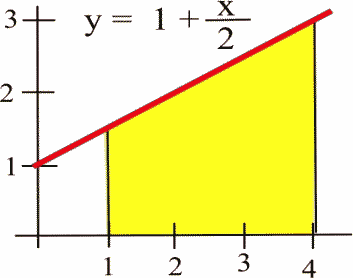
\includegraphics{images/image046.png}
\caption{}
\end{figure}

To view this video please enable JavaScript, and consider upgrading to a
web browser that \href{http://videojs.com/html5-video-support/}{supports
HTML5 video}

\hypertarget{second-derivative-test}{%
\subsection{Second Derivative Test}\label{second-derivative-test}}

Just as in the one-variable case, we'll need a way to test critical
points to see whether they are local max or min. There is a second
derivative test for functions of two variables that can help, but, just
as in the one-variable case, it won't always give an answer.

\hypertarget{the-second-derivative-test-for-functions-of-two-variables}{%
\paragraph{The Second Derivative Test for Functions of Two
Variables}\label{the-second-derivative-test-for-functions-of-two-variables}}

\begin{enumerate}
\item
  Find all critical points of \textbackslash{}(f(x,y)\textbackslash{}).
\item
  Compute \textbackslash{}{[}
  D(x,y)=\textbackslash{}left(f\_\{xx\}\textbackslash{}right)\textbackslash{}left(f\_\{yy\}\textbackslash{}right)-\textbackslash{}left(f\_\{xy\}\textbackslash{}right)\textbackslash{}left(f\_\{yx\}\textbackslash{}right),\textbackslash{}{]}
  and evaluate it at each critical point.

  \begin{enumerate}
  \item
    If \textbackslash{}(D \textbackslash{}gt 0\textbackslash{}), then
    \textbackslash{}(f\textbackslash{}) has a local max or min at the
    critical point. To see which, look at the sign of \textbackslash{}(
    f\_\{xx\} \textbackslash{}):

    \begin{itemize}
    \tightlist
    \item
      If \textbackslash{}( f\_\{xx\}\textbackslash{}gt 0
      \textbackslash{}), then \textbackslash{}(f\textbackslash{}) has a
      local minimum at the critical point.
    \item
      If \textbackslash{}( f\_\{xx\}\textbackslash{}lt 0
      \textbackslash{}), then \textbackslash{}(f\textbackslash{}) has a
      local maximum at the critical point.
    \end{itemize}
  \item
    If \textbackslash{}(D \textbackslash{}lt 0\textbackslash{}) then
    \textbackslash{}(f\textbackslash{}) has a saddle point at the
    critical point.
  \item
    If \textbackslash{}(D = 0\textbackslash{}), there could be a local
    max, local min, or neither (i.e., the test in inconclusive).
  \end{enumerate}
\end{enumerate}

To view this video please enable JavaScript, and consider upgrading to a
web browser that \href{http://videojs.com/html5-video-support/}{supports
HTML5 video}

\hypertarget{example-3}{%
\paragraph{Example 3}\label{example-3}}

Find all local maxima, minima, and saddle points for the function
\textbackslash{}{[} f(x,y)=x\^{}3+y\^{}3+3x\^{}2-3y\^{}2-8.
\textbackslash{}{]}

First we need the partial derivatives: \textbackslash{}( f\_x=3x\^{}2+6x
\textbackslash{}) and \textbackslash{}( f\_y=3y\^{}2-6y
\textbackslash{}).

Critical points are the places where both of these are zero (neither is
ever undefined): \textbackslash{}( f\_x=3x\^{}2+6x=3x(x+2)=0
\textbackslash{}) when \textbackslash{}(x = 0\textbackslash{}) or when
\textbackslash{}(x = -2\textbackslash{}). \textbackslash{}(
f\_y=3y\^{}2-6y=3y(y-2)=0 \textbackslash{}) when \textbackslash{}(y =
0\textbackslash{}) or when \textbackslash{}(y = 2\textbackslash{}).

Putting these together, we get four critical points: (0, 0), (-2, 0),
(0, 2), and (-2, 2).

Now to classify them, we'll use the Second Derivative Test. We'll need
all the second partial derivatives:
\textbackslash{}{[}f\_\{xx\}=6x+6,\textbackslash{}
f+\{yy\}=6y-6,\textbackslash{} f\_\{xy\}=f\_\{yx\}=0.\textbackslash{}{]}

Then \textbackslash{}{[} D(x,y)=(6x+6)(6y-6)-(0)(0)=(6x+6)(6y-6).
\textbackslash{}{]}

Now look at each critical point in turn:

\begin{itemize}
\tightlist
\item
  At (0, 0): \textbackslash{}( D(0,0)=(6(0)+6)(6(0)-6)=(6)(-6)=-36
  \textbackslash{}lt 0 \textbackslash{}), so there is a saddle point at
  (0, 0).
\item
  At (-2, 0): \textbackslash{}( D(-2,0)=(6(-2)+6)(6(0)-6)=(-6)(-6)=36
  \textbackslash{}gt 0 \textbackslash{}) and \textbackslash{}(
  f\_\{xx\}(-2,0)=6(-2)+6=-6 \textbackslash{}lt 0 \textbackslash{}), so
  there is a local maximum at (-2, 0).
\item
  At (0, 2): \textbackslash{}( D(0,2)=(6(0)+6)(6(2)-6)=(6)(6)=36
  \textbackslash{}gt 0 \textbackslash{}) and \textbackslash{}(
  f\_\{xx\}(0,2)=6(0)+6=6 \textbackslash{}gt 0 \textbackslash{}), so
  there is a local minimum at (0, 2).
\item
  At (-2, 2): \textbackslash{}( D(-2,2)=(6(-2)+6)(6(2)-6)=(-6)(6)=-36
  \textbackslash{}lt 0 \textbackslash{}), so there is another saddle
  point at (-2, 2).
\end{itemize}

To view this video please enable JavaScript, and consider upgrading to a
web browser that \href{http://videojs.com/html5-video-support/}{supports
HTML5 video}

\hypertarget{example-4}{%
\paragraph{Example 4}\label{example-4}}

Find all local maxima, minima, and saddle points for the function
\textbackslash{}{[} z=9x\^{}3+\textbackslash{}frac\{y\^{}3\}\{3\}-4xy.
\textbackslash{}{]}

We'll need all the partial derivatives and second partial derivatives,
so let's compute them all first: \textbackslash{}{[}
\textbackslash{}begin\{align*\} z\_x=\& 27x\^{}2-4y,\textbackslash{}quad
z\_y= y\^{}2-4x,\textbackslash{}\textbackslash{} z\_\{xx\}=\&
54x,\textbackslash{}quad z\_\{xy\}=z\_\{yx\}= -4,\textbackslash{}quad
z\_\{y\}= 2y. \textbackslash{}end\{align*\} \textbackslash{}{]}

Now to find the critical points: We need both \textbackslash{}( z\_x
\textbackslash{}) and \textbackslash{}( z\_y \textbackslash{}) to be
zero (neither is ever undefined), so we need to solve this set of
equations simultaneously: \textbackslash{}{[}
\textbackslash{}begin\{align*\} z\_x=\& 27x\^{}2-4y=0
\textbackslash{}\textbackslash{} z\_y=\& y\^{}2-4x=0
\textbackslash{}end\{align*\} \textbackslash{}{]}

Perhaps it's been a while since you solved systems of equations. One
solution method is the substitution method -- solve one equation for one
variable and substitute into the other equation: \textbackslash{}{[}
\textbackslash{}left.\textbackslash{}begin\{align*\} 27x\^{}2-4y=\& 0
\textbackslash{}\textbackslash{} y\^{}2-4x=\& 0
\textbackslash{}end\{align*\}\textbackslash{}right\textbackslash{}\}
\textbackslash{}to \textbackslash{}text\{Solve \textbackslash{}(
y\^{}2-4x=0 \textbackslash{}) for \textbackslash{}(
x=\textbackslash{}frac\{y\^{}2\}\{4\} \textbackslash{})
\textbackslash{}( \textbackslash{}dots \textbackslash{})\}
\textbackslash{}{]} \ldots{}then substitute into the other equation:
\textbackslash{}{[} \textbackslash{}begin\{align*\}
27\textbackslash{}left(\textbackslash{}frac\{y\^{}2\}\{4\}\textbackslash{}right)\^{}2-4y=\&
0 \textbackslash{}\textbackslash{}
\textbackslash{}frac\{27\}\{16\}y\^{}4-y=\& 0
\textbackslash{}end\{align*\} \textbackslash{}{]}

Now we have just one equation in one variable to solve. Factoring out a
\textbackslash{}(y\textbackslash{}) gives \textbackslash{}{[}
y\textbackslash{}left(\textbackslash{}frac\{27\}\{16\}y\^{}3-1\textbackslash{}right)=0,
\textbackslash{}{]} so \textbackslash{}( y=0 \textbackslash{}) or
\textbackslash{}( \textbackslash{}frac\{27\}\{16\}y\^{}3-1=0
\textbackslash{}), giving \textbackslash{}(
y=\textbackslash{}sqrt{[}3{]}\{\textbackslash{}frac\{1\}\{27/16\}\}=\textbackslash{}frac\{\textbackslash{}sqrt{[}3{]}\{4\}\}\{3\}
\textbackslash{}).

Plugging back in to the equation \textbackslash{}(
x=\textbackslash{}frac\{y\^{}2\}\{4\} \textbackslash{}) to find
\textbackslash{}(x\textbackslash{}) gives us the two critical points:
(0,0) and \textbackslash{}(
\textbackslash{}left(\textbackslash{}frac\{4\}\{9\},\textbackslash{}frac\{4\}\{3\}\textbackslash{}right)
\textbackslash{}).

Now to test them. First compute \textbackslash{}{[}
\textbackslash{}begin\{align*\} D(x,y)=\&
(f\_\{xx\})(f\_\{yy\})-(f\_\{xy\})(f\_\{yx\})
\textbackslash{}\textbackslash{} =\& (54x)(2y)-(-4)(-4)
\textbackslash{}\textbackslash{} =\& 108xy-16
\textbackslash{}end\{align*\} \textbackslash{}{]} Then evaluate
\textbackslash{}( D \textbackslash{}) at the two critical points:

\begin{itemize}
\tightlist
\item
  At (0,0): \textbackslash{}(D(0,0) = -16 \textbackslash{}lt
  0\textbackslash{}), so there is a saddle point at (0, 0).
\item
  At \textbackslash{}(
  \textbackslash{}left(\textbackslash{}frac\{4\}\{9\},\textbackslash{}frac\{\textbackslash{}sqrt{[}3{]}\{4\}\}\{3\}\textbackslash{}right)
  \textbackslash{}):
  \textbackslash{}(D\textbackslash{}left(\textbackslash{}frac\{4\}\{9\},\textbackslash{}frac\{\textbackslash{}sqrt{[}3{]}\{4\}\}\{3\}\textbackslash{}right)
  =16(\textbackslash{}sqrt{[}3{]}\{4\}-1) \textbackslash{}gt
  0\textbackslash{}), and \textbackslash{}(
  f\_\{xx\}\textbackslash{}left(\textbackslash{}frac\{4\}\{9\},\textbackslash{}frac\{\textbackslash{}sqrt{[}3{]}\{4\}\}\{3\}\textbackslash{}right)
  \textbackslash{}gt 0 \textbackslash{}), so there is a local minimum at
  \textbackslash{}(
  \textbackslash{}left(\textbackslash{}frac\{4\}\{9\},\textbackslash{}frac\{\textbackslash{}sqrt{[}3{]}\{4\}\}\{3\}\textbackslash{}right)
  \textbackslash{}).
\end{itemize}

\hypertarget{applied-optimization}{%
\subsection{Applied Optimization}\label{applied-optimization}}

To view this video please enable JavaScript, and consider upgrading to a
web browser that \href{http://videojs.com/html5-video-support/}{supports
HTML5 video}

\hypertarget{example-5}{%
\paragraph{Example 5}\label{example-5}}

A company makes two products. The demand equations for the two products
are given below. \textbackslash{}(p\_1\textbackslash{}),
\textbackslash{}(p\_2\textbackslash{}),
\textbackslash{}(q\_1\textbackslash{}),and
\textbackslash{}(q\_2\textbackslash{}) are the prices and quantities for
Products 1 and 2. \textbackslash{}{[} \textbackslash{}begin\{align*\}
q\_1=\& 200-3p\_1-p\_2 \textbackslash{}\textbackslash{} q\_2=\&
150-p\_1-2p\_2 \textbackslash{}end\{align*\} \textbackslash{}{]}

Find the price the company should charge for each product in order to
maximize total revenue. What is that maximum revenue?

Revenue is still price\textbackslash{}( \textbackslash{}cdot
\textbackslash{})quantity. If we're selling two products, the total
revenue will be the sum of the revenues from the two products:
\textbackslash{}{[} \textbackslash{}begin\{align*\} R(p\_1,p\_2)=\&
p\_1q\_1+p\_2q\_2 \textbackslash{}\textbackslash{} =\&
p\_1(200-3p\_1-p\_2)+p\_2(150-p\_1-2p\_2)
\textbackslash{}\textbackslash{} =\&
200p\_1-3p\_1\^{}2-2p\_1p\_2+150p\_2-2p\_2\^{}2
\textbackslash{}end\{align*\} \textbackslash{}{]}

This is a function of two variables, the two prices, and we need to
optimize it (just as in the previous examples). First we find critical
points. The notation here gets a bit hard to look at, but hang in there
-- this is the same stuff we've done before. \textbackslash{}{[}
R\_\{p\_1\}=200-6p\_1-2p\_2 \textbackslash{} \textbackslash{}text\{ and
\} \textbackslash{} R\_\{p\_2\}=150-2p\_1-4p\_2. \textbackslash{}{]}

Solving these simultaneously gives the one critical point
\textbackslash{}( (p\_1, p\_2)=(25,25) \textbackslash{})

To confirm that this gives maximum revenue, we need to use the Second
Derivative Test. Find all the second derivatives: \textbackslash{}{[}
R\_\{p\_1 p\_2\}=-6,\textbackslash{} R\_\{p\_2
p\_2\}=-4,\textbackslash{} \textbackslash{}text\{ and \}\textbackslash{}
R\_\{p\_1 p\_2\}=R\_\{p\_2 p\_1\}=-2. \textbackslash{}{]}

So \textbackslash{}( D(25,25)=(-6)(-4)-(-2)(-2) \textbackslash{}gt 0
\textbackslash{}) and \textbackslash{}( R\_\{p\_1 p\_2\}(25,25)
\textbackslash{}lt 0 \textbackslash{}), so this really is a local
maximum.

Thus, to maximize revenue the company should charge \$25 per unit for
both products. This will yield a maximum revenue of \$4375.

\begin{longtable}[]{@{}l@{}}
\toprule
\endhead
\href{section4-2.php}{← Previous Section}\tabularnewline
\bottomrule
\end{longtable}
